\begin{subfigure}[b]{0.4\textwidth}
    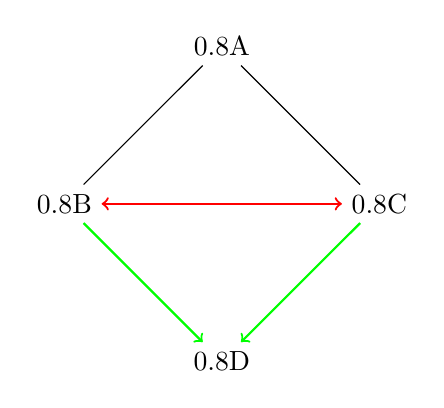
\begin{tikzpicture}
        \node (root) at (4,8) {\switch{0.8}{A}};
        \node (B) at (2,6) {\switch{0.8}{B}};
        \node (C) at (6,6) {\switch{0.8}{C}};
        \node (D) at (4,4) {\switch{0.8}{D}};

        \draw 
        (root) edge (B)
        (root) edge (C);

        \draw[green, thick, ->] 
        (B) edge (D)
        (C) edge (D);

        \draw[red, thick, <->]
        (B) edge (C);
    \end{tikzpicture}
    \caption{Broadcast is propagated}
\end{subfigure}
